
%
%  $Description: Author guidelines and sample document in LaTeX 2.09$ 
%
%  $Author: ienne $
%  $Date: 1995/09/15 15:20:59 $
%  $Revision: 1.4 $
%

\documentclass[times, 10pt,twocolumn]{article} 
\usepackage{latex8}
\usepackage{times}
\usepackage[utf8]{inputenc}
\usepackage{graphicx}
\usepackage{float}

%\documentstyle[times,art10,twocolumn,latex8]{article}

%------------------------------------------------------------------------- 
% take the % away on next line to produce the final camera-ready version 
\pagestyle{empty}

%------------------------------------------------------------------------- 
\begin{document}

\title{PADI-DSTM}

\maketitle
\thispagestyle{empty}

\begin{abstract}
   The ABSTRACT is to be in fully-justified italicized text, at the top 
   of the left-hand column, below the author and affiliation 
   information. Use the word ``Abstract'' as the title, in 12-point 
   Times, boldface type, centered relative to the column, initially 
   capitalized. The abstract is to be in 10-point, single-spaced type. 
   The abstract may be up to 3 inches (7.62 cm) long. Leave two blank 
   lines after the Abstract, then begin the main text. 
\end{abstract}

\Section{Introdução}
%Este artigo elaborado no âmbito da disciplina de Plataformas para Aplicações Distribuídas na Internet, tem como objectivo fazer uma apresentação e descrição da solução escolhida para a implementação do projecto \textit{PADI-DSTM}.

Inicialmente iremos abordar a nossa solução e compará-la com algumas alternativas que considerámos, apresentando uma vista global da sua arquitectura. De seguida falaremos das estruturas de dados e algoritmos escolhidos. Por fim, iremos abordar o trabalho a ser realizado posteriormente - tolerância a faltas - e iremos fazer uma pequena conclusão.

\section{Solução}

\subsection{2PC vs S2PL vs Timestamps}

Inicialmente considerámos seguir uma abordagem optimista. No entanto, como não sabemos qual é a relação existente entre o número de leituras e escritas, podemos admitir que existe igual número de leituras e escritas. Neste caso o número de conflitos existentes poderá ser grande. 

Considerando que isto seria um potencial bottleneck de performance no nosso sistema, optámos por abandonar as soluções que usam timestamps ou two-phase-commit (2PC). Para além disto outro argumento contra o 2PC é a possibilidade das transacções poderem abortar (se surgir algum conflito) depois de já terem realizado algum trabalho, o que implicaria refazer-se esse trabalho.

Assim, escolhemos utilizar \textit{Strict Two Phase Locking} ou \textit{S2PL}

\subsection{Replicação activa vs replicação passiva}

Depois de escolhermos qual o protocolo a usar, deparámo-nos com a escolha entre replicação activa e passiva. Inicialmente considerámos seguir replicação activa com um protocolo de \textit{Quorum Consensus}. No entanto, por esta precisar de três servidores (em vez dos dois necessários para a replicação passiva) e tendo também em conta que teríamos que enviar e receber mais mensagens do que as necessárias ao usar replicação passiva, optámos por esta última opção.



%%%%%%%
\section{Estruturas de Dados}

\subsection{Master}

Esta classe gere o sistema de memória distribuída e é responsável por armazenar os dados globais do sistema.

É importante salientar que a lista \textit{Servidores} tem como finalidade garantir que no caso em que o servidor primário for substituído, o endereço registado é actualizado e os clientes continuam a conseguir aceder aos \textit{PadInt}s sem perturbações. Para além disto, os \textit{TID} são atribuídos de forma sequencial e única. 

De seguida apresentam-se as estruturas internas desta classe.
\begin{table}[H]
\centering
\begin{tabular}{| p{2cm} | p{5cm} |}
\hline
\textbf{Variável} & \textbf{Descrição} \\
\hline
TID & Último \textit{Transaction ID} atribuído \\
\hline
Servidores & Estrutura que mapeia o identificador de cada servidor primário com o seu endereço \\
\hline
\end{tabular}
\caption{Atributos da classe Master}
\end{table}


\subsection{Servidor}
O conjunto das instâncias da classe Servidor representa a memória distribuída onde são armazenados os \textit{PadInt}s. De seguida apresentam-se os atributos desta classe.
\begin{table}[H]
\centering
\begin{tabular}{| p{2cm} | p{5cm} |}
\hline
\textbf{Variável} & \textbf{Descrição} \\
\hline
Pedidos & Lista de pedidos feitos ao servidor enquanto o servidor está no modo \textit{Freeze} \\
\hline
Réplica & Endereço do outro servidor \\
\hline
Valor original & Estrutura que mapeia \textit{UID}s em \textit{PadInt}s \\
\hline
\end{tabular}
\caption{Atributos da classe Servidor}
\end{table}

A localização de cada \textit{PadInt} depende do número total de servidores primários, ou seja, é dada por:

\centerline{\textit{UID} \textbf{mod}  \textit{Nº de Servidores}}

\subsection{PadInt}

Esta classe representa o objecto gerido pelo \textit{PADI-DSTM} que guarda um inteiro, onde o \textit{lock} é apenas o TID. Esta classe é composta por:
\begin{table}[H]
\centering
\begin{tabular}{| p{2cm} | p{5,5cm} |}
\hline
\textbf{Variável} & \textbf{Descrição} \\
\hline
UID & Identificador do inteiro que representa \\
\hline
Valor actual & Valor no momento actual da transacção \\
\hline
Valor original & Valor no início da transacção \\
\hline
Temporizador & Usado na detecção de deadlocks \\
\hline
Promoção & Referência para a próxima transação a ser promovida\\
\hline
Leitores & Fila de transacções com locks de leitura atribuídos \\
\hline
Escritor & Transacção com lock de escrita atribuído\\
\hline
Leitores à espera & Fila de transações com locks de leitura à espera \\
\hline
Escritores à espera & Fila de transações com locks de escrita à espera\\
\hline
\end{tabular}
\caption{Atributos da classe PadInt}\label{tab:padint}
\end{table}


\subsection{Stub do PadInt}

A Biblioteca envia ao cliente stubs da classe \textit{PadInt}. Esta classe tem a seguinte estrutura:

\begin{table}[H]
\centering
\begin{tabular}{| p{2cm} | p{5,5cm} |}
\hline
\textbf{Variável} & \textbf{Descrição} \\
\hline
UID & Identificador do inteiro que representa \\
\hline
Biblioteca & Referência para a Biblioteca do Cliente \\
\hline
\end{tabular}
\caption{Atributos da classe Master}
\end{table}

Esta classe exporta os seguintes métodos:

\begin{itemize}
	\item \textit{int Read()}: Invoca o método \textit{Read} da Biblioteca
	\item \textit{void Write(int value)}: Invoca o método \textit{Write} da Biblioteca
\end{itemize}

\subsection{Biblioteca}
Esta é a classe que representa a biblioteca usada pelos clientes para comunicar com o sistema de memória distribuida. Esta classe tem a seguinte estrutura:

\begin{table}[H]
\centering
\begin{tabular}{| p{2,1cm} | p{5cm} |}
\hline
\textbf{Variável} & \textbf{Descrição} \\
\hline
Nº de Servidores & Número total de servidores primários existentes  \\
\hline
TID & Transacção atribuída pelo \textit{Master} \\
\hline
(UID, Servidor) & Lista de associações entre \textit{UID}s e o seu respectivo \textit{Servidor} \\
\hline
Cache de Servidores & Estrutura que mapeia \textit{UID} no \textit{Servidor} em que o \textit{PadInt} está armazenado \\
\hline
Temporizadores & Lista de \textit{timers} para cada servidor \\
\hline
\end{tabular}
\caption{Atributos da classe Biblioteca} \label{lib}
\end{table}
%%%%%%%%

\section{Algoritmos propostos}

\subsection{Locking}

\subsubsection{obterLockEscrita(TID, UID)}

\begin{figure}[H]
\centering
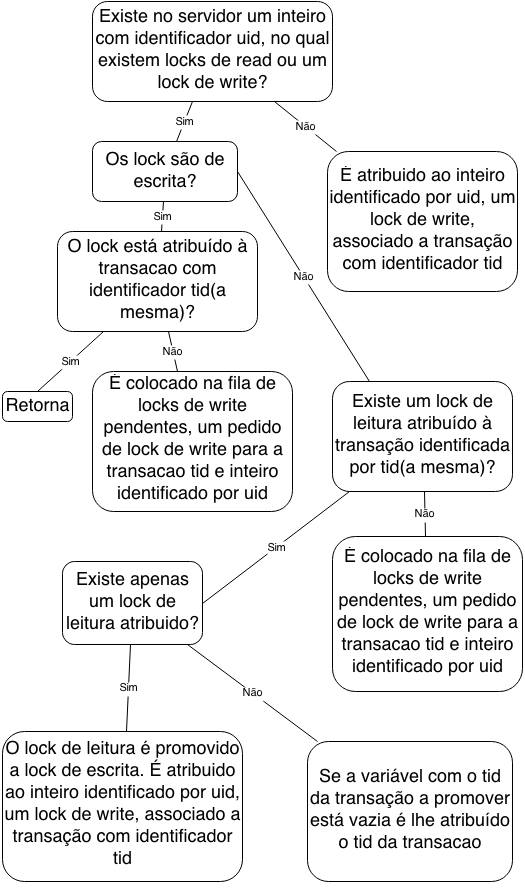
\includegraphics[width=6.75cm]{obtem_lock_w.jpg}
\caption{Obtenção de locks de escrita}
\end{figure}

\subsubsection{obterLockLeitura(TID, UID)}
Caso não exista no servidor um \textit{lock} de leitura ou escrita sobre o \textit{PadInt} identificado pelo \textit{UID} atribuído à transacção com \textit{TID}, verifica-se se existe um \textit{lock} de escrita e se existir é posto na variável \textit{Leitores à espera} o \textit{TID}. Caso contrário é atribuído à transacção um \textit{lock} de leitura do \textit{PadInt}.

\subsubsection{libertarLockEscrita(TID, UID)}

O servidor remove o \textit{lock} de escrita da transacção identificada por \textit{TID}, associada ao PadInt identificado por \textit{UID}.

É invocado o método \textit{tiraQueueEscrita(UID)}, para que outras transações possam associar outros locks ao PadInt.

\subsubsection{tiraQueueEscrita(UID)}

Se no \textit{PadInt} identificado pelo \textit{UID}, existir na variável \textit{Promoção} uma transacção a promover, essa transacção é removida da fila e é invocado o método \textit{obterLockEscrita(TID,UID)}. Caso contrário, é verificado se existe na fila de \textit{locks} de escrita pendentes do \textit{UID} alguma transacção pendente:
\begin{itemize}
	\item Se existir, o \textit{TID} dessa transacção é removida da fila e é invocado o método \textit{obterLockEscrita(TID,UID)}. 
	\item Se não existir e se existe na fila de \textit{locks} de read pendentes algum \textit{TID}  que esteja associado a \textit{UID}, esse \textit{TID} é removido da fila e é invocado o método \textit{obterLockLeitura(TID,UID)}.
\end{itemize}

\subsubsection{libertarLockLeitura(TID, UID)}

O servidor remove o \textit{lock} de leitura, da transacção identificada pelo \textit{TID}, associada ao \textit{PadInt} identificado por \textit{UID}.

É invocado o método \textit{tiraQueueLeitura(UID)}, para que outras transações possam associar outros locks ao PadInt.

\subsubsection{tiraQueueEscrita(UID)}

No método \textit{tiraQueueLeitura(UID)} verifica-se se existe um único \textit{lock} de read associado ao \textit{PadInt} identificado por \textit{UID} e caso exista, na variável \textit{Promoção} algum \textit{TID} pendente, esse \textit{TID} é removido e é invocado o método \textit{obterLockEscrita(TID,UID)}. No caso em que não existe nenhum \textit{TID} na variável \textit{Promoção}, mas existe alguma transação na variável \textit{Escritores à espera} é removido uma transacção dessa variável e é invocado o método \textit{obterLockEscrita(TID,UID)}.

\subsubsection{escrevePadInt(TID, UID, value)}

Este método chama o método \textit{obterLockEscrita(TID, UID)} e quando o \textit{lock} de escrita é colocado na variável \textit{Escritor}, o valor é escrito. De seguida é retornado um \textit{ack} à Biblioteca. No caso em que ocorre um abort devido ao um deadlock é lançada uma excepção.

\subsubsection{lePadInt(TID, UID)}

Este método chama o método \textit{obterLockLeitura(TID, UID)} e quando o \textit{lock} de leitura é colocado na variável \textit{Leitores}, o valor do \textit{PadInt} é lido, sendo depois retornado à Biblioteca. No caso em que ocorre um abort devido a um deadlock é lançada uma excepção
\subsection{Commit}

Quando é invocado o método TxCommit, são percorridos os pares \textit{(UID, servidor)} na estrutura descrita na Tabela~\ref{lib}, enviando a cada servidor primário um pedido para que faça commit de todos os \textit{PadInts} que foram acedidos para leitura ou escrita durante o decorrer da transação atual.

Ao receber o pedido de commit, o servidor primário percorre a lista de identificadores de \textit{PadInt}s envolvidos no commit e, para cada um deles, verifica se o \textit{TID} recebido como argumento pertence a alguma das seguintes variáveis da classe \textit{PadInt} ilustradas na Tabela~\ref{tab:padint}: Leitores, Escritor, Leitores à espera, Escritores à espera, Promoção.

Se \textit{TID} que identifica a transacção estiver contido nalguma das variáveis acima descritas, este é removido dessa variável. É também criado e guardado um par \textit{(TID, Boolean\footnote{O boolean indica se o commit teve sucesso ou não})}. Este par é usado se eventualmente o servidor primário entrar no estado de \textit{Fail}, o secundário assumir o papel de primário e a \textit{Lib} lhe pedir para responder a um commit/abort de uma transacção terminada, mas à qual o primário (agora em modo \textit{Fail}), nunca chegou a enviar uma mensagem de \textit{ack}.

Se o \textit{TID} não pertence a nenhuma das variáveis anteriormente descritas e o \textit{TID} da transacção a ser tratada é o mesmo que foi registado da última vez que se guardou um par (tid, valor final atribuido a um PadInt) no final da ultima transacção, então o valor registado no par como resultado final da transacção é devolvido como retorno à lib e o par é apagado.

O servidor primário faz o pedido ao servidor secundário para que execute o commit, invocando o mesmo método com os mesmos argumentos. Depois de executar o pedido do primário, o secundário envia um \textit{ack} ao primário a confirmar que executou o método.

O servidor primário recebe a mensagem de \textit{ack} do secundário e reporta à Biblioteca o sucesso da execução do commit.

É importante referir que no passo em que são removidos os \textit{locks}, a motivação para se verificar se o \textit{TID} se encontra na lista de variáveis acima referidas e não apenas nas variáveis \textit{Leitores} e \textit{Escritor}, prende-se com o facto de não existir nenhuma forma de impedir que o cliente tente obter locks e tente faça commit ou abort à transacção antes sequer de os ter obtido.
\subsection{Recuperação de aborts}
\subsection{Detecção de deadlocks}

Para a detecção de deadlocks usámos um temporizador para cada \textit{PadInt} existente no servidor. Este temporizador é activado quando se coloca um pedido em espera, seja para promoção de lock ou para obter lock de escrita/leitura. Quando o temporizador expira é feito abort da transação\footnote{Admitindo que existem mais transacções à espera de serem promovidas ou para lerem/escreverem} (ou transações no caso de existirem locks de leitura atribuídos) que possuía o lock e escolhe-se um pedido dos que estão em espera para ser executado pela seguinte ordem: pedido de promoção, pedido de lock de escrita e finalmente pedido de lock de leitura.


%%%%%%%%%%%%
\section{Tolerância a Faltas}

\subsection{Fail}

\subsection{Freeze}

\section{Conclusão}

\nocite{ex1,ex2}
\bibliographystyle{latex8}
\bibliography{latex8}

\end{document}

